\section[Plus d'humains, plus de chats, moins de machines]{Plus d'humains, plus de chat, moins de machines}

\subsection{Moins de machines, moins d'algorithme, plus d'humains}

\begin{frame}{Des acteurs pour des internets plus respectueux (1/2)}
  \begin{center}
    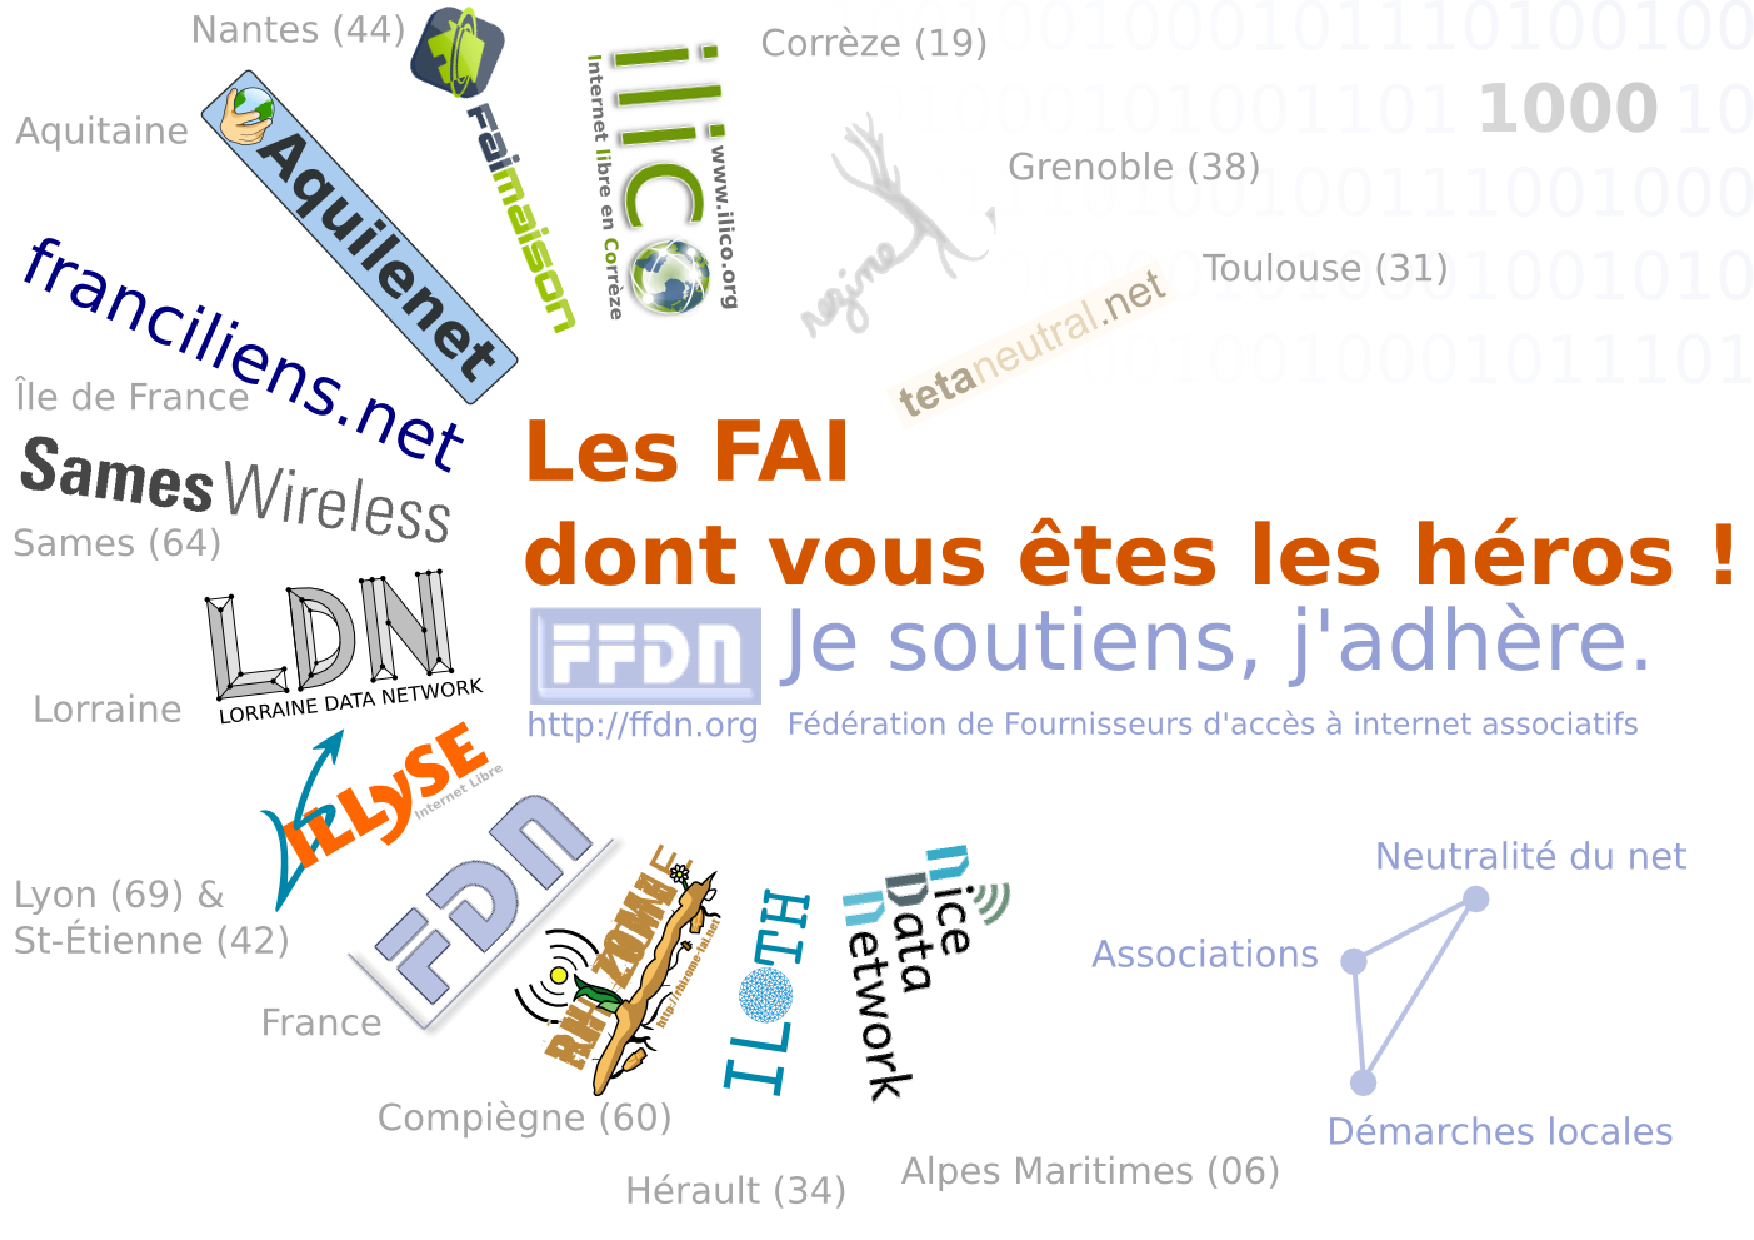
\includegraphics[height=0.8\textheight]{un_autre_internet/les_fai_dont_vous_etes.pdf}
  \end{center}
\end{frame}

\begin{frame}{Des acteurs pour des internets plus respectueux (2/2)}
  \begin{columns}
    \begin{column}{0.5\textwidth}
      
\includegraphics[height=0.2\textheight]{un_autre_internet/hadoly.png}
      
\includegraphics[height=0.2\textheight]{un_autre_internet/framasoft.png}
    \end{column}
    \begin{column}{0.5\textwidth}
    \begin{center}
      \includegraphics[height=0.8\textheight]{un_autre_internet/chatons.png}
    \end{center}
    \end{column}
  \end{columns}
\end{frame}

\begin{frame}{Des volontés communes}
  La neutralité du net, Rester humain et local
  Mettre un illustration
\end{frame}

\subsection{Les CHATONS: Hadoly}

\begin{frame}{Hadoly: Hébergeur Associatif Décentralisé et Ouvert à Lyon}
  TODO présentation d'hadoly
\end{frame}

\begin{frame}{Hadoly: Des services ouverts à tous}
  TODO présentation des services ouverts
  mettre un screen de pads
\end{frame}

\begin{frame}{Hadoly: C'est aussi des mails}
  TODO présentation du service des mails
  mettre un screen de mail hadoly
\end{frame}

\begin{frame}{Hadoly: Un cloud}
  TODO présentation du service de clouds
  mettre un screen de mail hadoly
\end{frame}

\begin{frame}{Hadoly: Et bien d'autres}
  TODO présentation des autres services (git, projet, support)
  mettre un screen d'un des services
\end{frame}

\subsection{Les FAI Associatif: Illyse}

\begin{frame}{Illyse: Internet Libre sur Lyon et Saint-Etienne}
  TODO présentation d'Illyse
  mettre photo/screen, à voir
\end{frame}

\begin{frame}{Illyse: De l'xDSL ...}
  TODO présentation du service xDSL
  mettre une illustration
\end{frame}

\begin{frame}{Illyse: \hfill ... Du VPN ...\hfill}
  TODO présentation du services VPN
  mettre une illustration
\end{frame}

\begin{frame}{Illyse: \hfill ... Et de la fibre}
  TODO présentation du projet fibre dans la loire
\end{frame}

\begin{frame}{Convaincu ? Alors rejoignez-nous}
  Faisons des internets un monde plus humains mais avec toujours autant de chats !
:
  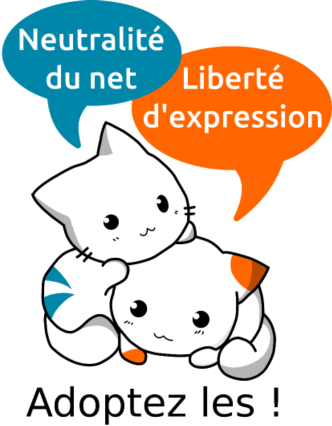
\includegraphics[height=0.7\textheight]{un_autre_internet/adoptez_les.png}
\end{frame}

% vim: ts=2: sw=2: sts=2
